\hide{
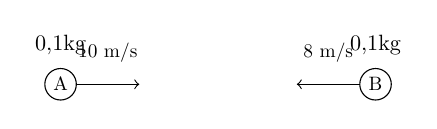
\begin{tikzpicture}
\foreach \x /\y/\z in {0/A/{0,1kg},4/B/{0,1kg}} {
\draw (\x,0) circle (0.2) node[scale=0.7]{\y};
\node at (\x,0.5) [scale=0.8]{\z};}
\draw[->] (0.2,0)--node[midway, yshift=0.4cm,scale=0.7]{10 m/s}(1,0);
\draw[->] (3.8,0)--node[midway, yshift=0.4cm,scale=0.7]{8 m/s}(3,0);
\end{tikzpicture}

Diketahui:

\begin{tabular}{p{0.5cm} p{1mm} p{2cm} p{1cm} p{0.5cm} p{2cm} }
$m_A$ &= &0.1 kg  & & &\\
$m_B$ &= &0.1 kg  & & &\\
$v_A$ &= &10 m/s  & & &\\
$v_B$ &= &-8 m/s  & & &\\
$e$ &= &1  & & &\\
\end{tabular}

Ditanya : $v_A'$ atau $v_1'$ dan $EK_A'$ ?

Jawab:

Karena lenting sempurna maka berlaku
\begin{align*}
e &= \frac{-(v_2'-v_1')}{v_2-v_1}\\
1 &= \frac{-v_2'+v_1'}{-8-(10)}\\
1 &= \frac{-(v_2'-v_1')}{-18}\\
\coret{-}18 &= \coret{-}(v_2'-v_1')\\
18 &= v_2' -v_1'
\end{align*}
Berlaku pula persamaan kekekalan momentum, massa sama
\begin{align*}
\Sigma p &= \Sigma p\\
\coret{m_A}v_1 + \coret{m_B}v_2 &= \coret{m_A}v_1' + \coret{m_B}v_2' \\
10-8 &= v_1' + v_2'\\
2 &= v_1' + v_2'
\end{align*}}
\hide{
Kemudian proses eliminasi sehingga 
\begin{align*}
18 &= v_2' -v_1'\\
2 &= v_2' + v_1'\\
\text{----}&\text{----------------(-)}\\
16 &=-2v_1'\\
v_1' &= -8 \text{ m/s}
\end{align*}
energi Kinetiknya $\frac{1}{2}mv^2=3,2$ J

Jika mereka \textbf{MASSA SAMA dan LENTING SEMPURNA} maka hanya bertukar kecepatan. Sehingga $v_1'=v_2=-8$ dengan arah ke kiri. }
sapi
